\section{Big Data Analytics - I Lecture}

\subsection{Introduction to Big Data
    Analytics}\label{introduction-to-big-data-analytics}

Good morning, everyone. Today's class is focused on Big Data Analytics.
Let me share my screen so you can follow along with the slides. Big Data
Analytics is a widely discussed topic these days, and it's important to
understand what it truly entails and the opportunities it presents for
businesses. We will also explore how technology has evolved and how this
evolution has shaped the applications of Big Data Analytics. To
illustrate these concepts, we will examine a few case studies.


\subsection{Defining Key Terms}\label{defining-key-terms}

\begin{figure}[!h]
    \centering
    \includegraphics[page=4, trim = 1.5cm 4cm 1.5cm 4cm, clip, width=\textwidth]{images/06 - BIG_DATA.pdf}
\end{figure}

\subsubsection{Artificial Intelligence}\label{artificial-intelligence}

In order to establish a common vocabulary for this class, let's begin by
defining some key terms. While many of you, as computer engineering
students, may already be familiar with these definitions from previous
courses, it's important to ensure that everyone, including management
engineering and telecommunication engineering students, understands the
terms we will be using.

First and foremost, let's define artificial intelligence (AI). AI refers
to the intelligence exhibited by machines, in contrast to the natural
intelligence displayed by humans and other animals. It encompasses the
intelligence demonstrated by machines.


\subsubsection{Machine Learning}\label{machine-learning}

Machine learning is a subset of artificial intelligence (AI), meaning
that AI encompasses more than just machine learning. Machine learning is
a specific type of AI where computers learn to solve problems based on
data, without the need for explicit programming or predefined rules.
This ability to learn and solve problems without code has made machine
learning highly popular in recent years. It offers companies the
opportunity to develop useful applications of information technology
without the need for extensive coding. This is particularly appealing
considering the shortage of skilled computer engineers. Machine learning
allows organizations to leverage the data they have collected over the
years and apply it to various IT applications. While machine learning
receives a lot of attention, it's important to remember that it is only
a small part of the broader field of artificial intelligence.


\subsubsection{Problems and Capabilities of
    AI}\label{problems-and-capabilities-of-ai}

\begin{figure}[!h]
    \centering
    \includegraphics[page=5, trim = 1.5cm 3cm 1.5cm 4cm, clip, width=\textwidth]{images/06 - BIG_DATA.pdf}
\end{figure}

Let me provide you with some examples of the common problems and
capabilities associated with artificial intelligence (AI). Problems that
AI aims to address include reasoning, knowledge representation,
planning, learning, natural language processing (NLP), robotics for
object manipulation, and perception for sensor development. On the other
hand, the capabilities typically classified as AI encompass
understanding human speech, competing in strategic games like chess and
Go, autonomous driving, intelligent content delivery networks, military
simulations, and many more. These examples only scratch the surface of
the numerous applications of AI.


\subsubsection{Classes of Machine Learning
    Algorithms}\label{classes-of-machine-learning-algorithms}

\begin{figure}[!h]
    \centering
    \includegraphics[page=6, trim = 1.5cm 4cm 1.5cm 4cm, clip, width=\textwidth]{images/06 - BIG_DATA.pdf}
\end{figure}

In the field of machine learning, algorithms are typically categorized
into two main classes: unsupervised and supervised. While there are also
semi-supervised algorithms, for the sake of simplicity, let's focus on
the distinction between supervised and unsupervised learning.

Unsupervised learning algorithms have the ability to learn how to solve
a specific problem by analyzing the data, without the need for a
predefined correct solution. On the other hand, supervised learning
algorithms require a set of problem instances along with their
corresponding correct solutions, which is known as the ``ground truth.''
In supervised learning, algorithms need explicit feedback to determine
whether they are solving specific instances of the problem correctly or
incorrectly.

The ground truth, therefore, refers to the set of problem instances and
their correct solutions that are used to train supervised learning
algorithms. It serves as a reference for the algorithm to learn from and
improve its performance. However, the reliance on the ground truth is
one of the main limitations of applying machine learning in real-world
scenarios.


\subsubsection{Ground Truth and Its
    Importance}\label{ground-truth-and-its-importance}

Obtaining ground truth can be a challenge for companies, as they may
have plenty of data but lack the actual solution to the problem
instances. The question then becomes how to collect the necessary ground
truth. In most cases, the ground truth is obtained through direct
measurement of real-world data. For example, if you need pictures of
tanks, you can use a drone to capture those pictures, ensuring that they
are labeled as tanks. However, collecting ground truth can be costly in
terms of time and effort for companies. In some cases, the cost of
collecting ground truth is so high that even though machine learning
could be beneficial in theory, it may not be feasible to apply it due to
the challenges associated with obtaining the necessary ground truth.


\subsubsection{Case Study: Crop
    Classification}\label{case-study-crop-classification}

\begin{figure}[!h]
    \centering
    \includegraphics[page=7, trim = 1.5cm 1cm 1.5cm 4.8cm, clip, width=\textwidth]{images/06 - BIG_DATA.pdf}
\end{figure}

Let's consider the case study of crop classification in the context of
earth observation. Satellites regularly capture images of the Earth,
dividing them into pixels, each with its own color. The challenge is to
determine the type of crop cultivated in each pixel based on its color.
While machine learning algorithms can be used for this task, obtaining
labeled data, or ground truth, is essential.

There are two approaches to obtaining ground truth. The first is
supervised learning, where pixels are labeled with the corresponding
crop type. This requires a significant amount of labeled data to train
the algorithm effectively. The second approach is unsupervised learning,
where pixels are grouped based on similarity. However, the crop type for
each group is unknown. To assign labels to the grouped pixels, at least
one pixel in the cluster must be observed and labeled.

While unsupervised learning can be performed without any ground truth,
having some labeled observations is necessary to make the application
useful. With supervised learning, a larger amount of accurately labeled
data is required. However, the precision achieved with supervised
learning is often superior to that of unsupervised learning.

Collecting ground truth for crop classification can be expensive and
time-consuming, as it involves physically visiting fields to observe the
crops. However, the benefits of accurate crop classification are
significant. For example, in finance, crop classification can help make
investment decisions based on projected crop availability and estimated
prices. This information allows investors to determine whether and at
what price to invest.

In conclusion, while collecting ground truth for crop classification may
be costly, the value and usefulness of the application make it
worthwhile. Accurate crop classification enables informed
decision-making in various industries, such as finance.

In many finance-related applications, collecting the ground truth is
essential because these applications generate significant revenue. There
are professionals who specialize in collecting the ground truth for
these applications. However, this is not always the case for all
applications. Some applications may not generate enough revenue to
justify the effort and cost of collecting the ground truth.

\subsection{Deep Learning}\label{deep-learning}

\begin{figure}[!h]
    \centering
    \includegraphics[page=8, trim = 1.5cm 5.5cm 1.5cm 4cm, clip, width=\textwidth]{images/06 - BIG_DATA.pdf}
\end{figure}

Now, let's move on to understanding what deep learning is. Deep learning
is a specific subset of machine learning, which itself is a subset of
artificial intelligence. In deep learning, algorithms consist of
multiple layers of nonlinear nodes that process input data to produce an
output, which represents the solution to a given problem. The input data
describes the problem, while the output is the desired solution.

\begin{figure}[!h]
    \centering
    \includegraphics[page=9, trim = 1.5cm 2cm 1.5cm 4cm, clip, width=\textwidth]{images/06 - BIG_DATA.pdf}
\end{figure}

The diagram represents a multi-layer neural network, where each node
represents a nonlinear function. The network consists of input nodes,
output nodes, and intermediate layers where the input data passes
through nonlinear functions and is then forwarded to subsequent nodes.
The final layer, in this case, is layer three, which generates the
output. The nodes in the network have parameters associated with them,
and during training, these parameters are adjusted to optimize the
network's output with minimal error.

Neural networks are known to require a large amount of input data with
known correct outputs for training. Considering the number of nodes,
connections, and parameters in the network, it becomes clear why
collecting the ground truth is a significant challenge. Many instances
of problems with their corresponding correct solutions are needed to
train the network effectively and find the best combination of
parameters that produce the desired output.


\subsection{Natural Language Processing
    (NLP)}\label{natural-language-processing-nlp}

\begin{figure}[!h]
    \centering
    \includegraphics[page=10, trim = 1.5cm 5cm 1.5cm 4cm, clip, width=\textwidth]{images/06 - BIG_DATA.pdf}
\end{figure}

\subsubsection{Evolution and
    Applications}\label{evolution-and-applications}

There are various mechanisms and algorithms, such as one-shot learning,
few-shot learning, and extreme machine learning, that aim to reduce the
amount of input required to obtain the desired output. Additionally,
strategies like ground truth augmentation and synthetic data can be used
to make the most of limited instances or generate instances when none
are available. However, these approaches are still the subject of
ongoing research.

\begin{figure}[!h]
    \centering
    \includegraphics[page=11, trim = 1.5cm 5cm 1.5cm 4cm, clip, width=\textwidth]{images/06 - BIG_DATA.pdf}
\end{figure}

Moving on to natural language processing (NLP), it focuses on enabling
humans and computers to interact using natural language, such as spoken
or written language, without the need for humans to adapt to computer
language. NLP has gained attention in various fields over the years. In
the 1990s, it was primarily used for document management,
classification, retrieval, and topic extraction. Around the year 2000,
it expanded to include document and web search, exemplified by Google.
In 2005, speech-to-text capabilities were developed. From 2010 onwards,
NLP has been applied to social media analytics, reputation management,
sentiment analysis, and more recently, chatbots.

Despite these advancements, it is important to note that NLP is not yet
a fully mature field. There are still many areas where further work is
needed to ensure optimal performance. For example, sentiment analysis
remains a challenging task, as there is currently no tool that can
automate sentiment analysis with sufficient accuracy across different
contexts.


\subsubsection{Chatbots and Their
    Effectiveness}\label{chatbots-and-their-effectiveness}

\begin{figure}[!h]
    \centering
    \includegraphics[page=12, trim = 1.5cm 3.3cm 1.5cm 4cm, clip, width=\textwidth]{images/06 - BIG_DATA.pdf}
\end{figure}

In the realm of Natural Language Processing (NLP), there is still much
work to be done for chatbots to reach their full potential. While there
have been advancements in NLP over the past decade, even older
applications require further development. Chatbots, in particular, are
still in their early stages. To gain insight into what companies are
currently doing in this field, you can watch the video provided in the
link on this slide.

Currently, our experience with chatbots is limited in terms of NLP
capabilities. Ideally, in NLP, we should be able to interact with
chatbots through speech or written text, and they should understand and
provide relevant answers. However, most chatbots today initiate the
conversation by asking questions, guiding users through a predefined
interface with buttons to press. This approach does not effectively
address the user's specific problem or needs. In my opinion, these
chatbots are not very effective.

If you start asking questions and the chatbot fails to provide immediate
answers or if you express dissatisfaction, it is possible that a human
operator will intervene. The system recognizes when the chatbot is not
effectively interacting with the user and prompts a human to take over.
This approach is similar to the concept of call centers, where
automation directs queries to the appropriate operator and handles
common questions. If automation fails, a human operator steps in. It's
important to note that in most cases, we are not referring to chatbots
that can understand spoken language.

In the early days of chatbots, there was not even an interface to
indicate that user input was required. Users were allowed to start
asking questions right away, but unfortunately, the chatbot often
provided incorrect answers. Even if the user asked a common question
that the chatbot should have been able to answer, the challenge lies in
understanding the user's specific phrasing. There are countless ways to
ask about the opening hours of a shop, for example, and the chatbot must
be able to extract the meaning regardless of the specific wording.
However, we are still far from achieving this level of understanding.

The paradigm of chatbots represents an interesting inversion of
traditional approaches.


\subsubsection{Inversion of Paradigm in Mobile
    Apps}\label{inversion-of-paradigm-in-mobile-apps}

\begin{figure}[!h]
    \centering
    \includegraphics[page=13, trim = 1.5cm 1.7cm 1.5cm 3.5cm, clip, width=\textwidth]{images/06 - BIG_DATA.pdf}
\end{figure}

The "inversion of paradigm" in mobile apps refers to a shift in how users interact with their devices. Traditional apps require manual interaction: opening the app, navigating through menus, and inputting information. The inverted paradigm, however, utilizes chatbots to streamline the process, allowing users to engage in a more natural, conversational manner to achieve their goals

For example, you can ask the chatbot to open your diet mobile app and
tell you how many calories you have left for the day, or inquire about
your fat intake or the number of steps you've taken. You can even ask
the chatbot to perform calculations like extracting the square root of a
number. The chatbot acts as your intermediary, connecting with the
mobile apps through APIs (Application Programming Interfaces) to perform
the requested tasks automatically, without the need for you to navigate
through app interfaces.

In this way, the chatbot becomes the sole interface, the one-stop-shop
for interacting with all your mobile apps. It simplifies the user
experience by providing a single point of interaction. However, for this
to work, two things are necessary. Firstly, the chatbot needs to be
embedded in the operating system with APIs. Secondly, the mobile apps
themselves need to utilize these APIs to enable interaction with the
chatbot. While some progress has been made in this direction, there is
still a long way to go.

\begin{figure}[!h]
    \centering
    \includegraphics[page=14, trim = 1.5cm 4cm 1.5cm 4.5cm, clip, width=\textwidth]{images/06 - BIG_DATA.pdf}
\end{figure}

\begin{figure}[!h]
    \centering
    \includegraphics[page=15, trim = 1.5cm 3cm 1.5cm 5cm, clip, width=\textwidth]{images/06 - BIG_DATA.pdf}
\end{figure}

To illustrate this concept, let's take a look at the chatbots developed
by La Republica and Sky Scanner. These chatbots have shown promising
capabilities, although there is still room for improvement.

\begin{figure}[!h]
    \centering
    \includegraphics[page=16, trim = 1.5cm 2cm 1.5cm 3.3cm, clip, width=\textwidth]{images/06 - BIG_DATA.pdf}
\end{figure}

\paragraph{PAMela chatbot}
In terms of interaction, the chatbot primarily relies on button clicks
rather than typing or voice input. Through our research with a
supermarket called PAM, we identified the most common questions asked by
clients that could be answered by a chatbot. We then worked on
envisioning different ways these questions could be asked, ensuring that
the bot could effectively respond to text-based queries without the need
for a specific interface or voice input.

To create an effective chatbot, it is crucial to address a broad range
of questions. However, we found that allowing customers the freedom to
ask questions in their own natural language poses a significant
challenge. We are continuously working on improving this aspect.

\subsection{Privacy Concerns and
    Technology}\label{privacy-concerns-and-technology}


\begin{figure}[!h]
    \centering
    \includegraphics[page=17, trim = 1.5cm 1cm 0.7cm 1cm, clip, width=\textwidth]{images/06 - BIG_DATA.pdf}
\end{figure}

It is worth mentioning popular voice assistants like Alexa, Google Home,
and Google Assistant. These platforms allow companies to connect and
provide services through voice interactions, simplifying the user
experience. However, relying on these third-party technologies means
sacrificing some privacy. These technologies gather extensive
information about users, raising concerns about data security and
privacy. In Europe, where such technologies are not as prevalent, the
General Data Protection Regulation (GDPR) aims to mitigate privacy risks
for users.


\subsection{Applications of Machine Learning and AI in
    Industry}\label{applications-of-machine-learning-and-ai-in-industry}


\begin{figure}[!h]
    \centering
    \includegraphics[page=19, trim = 0cm 1.5cm 1.5cm 0.7cm, clip, width=\textwidth]{images/06 - BIG_DATA.pdf}
\end{figure}

This chart presents the most prevalent applications of machine learning
and AI, based on a survey conducted with managers in various industries
such as agriculture, banking, healthcare, and manufacturing. Take a
moment to review this slide and gain insight into the current priorities
of managers. Among the recurring services, two stand out: predictive
maintenance in manufacturing and targeted services. These applications
are widely recognized as the most common and in-demand. While there are
other applications available, these two are considered the hottest and
most frequently implemented. Many companies have already conducted pilot
projects in these areas to assess the potential benefits and understand
the associated challenges of applying machine learning.


\subsection{Automating Decision Making with Machine
    Learning}\label{automating-decision-making-with-machine-learning}


\begin{figure}[!h]
    \centering
    \includegraphics[page=20, trim = 1.5cm 2.5cm 2.5cm 2.9cm, clip, width=\textwidth]{images/06 - BIG_DATA.pdf}
\end{figure}


In general, machine learning is used to embed decision-making
capabilities into various applications. For instance, in predictive
maintenance, machine learning helps determine the optimal timing for
executing maintenance interventions. However, it is crucial to define
what ``optimal'' means in this context. It could refer to reducing
maintenance costs, minimizing the number of interventions, or improving
the quality of service. To ensure effective decision-making, it is
essential to associate the appropriate key performance indicators (KPIs)
with machine learning.

One significant aspect of machine learning applications is that they
automate decision-making processes. Instead of human decision-makers,
machines are responsible for making decisions. This automation is what
sets machine learning apart from traditional IT applications. When
exploring different machine learning applications, it becomes evident
that decision-making is a fundamental component of each one.

The novelty of machine learning lies in the fact that decisions are
automated. Unlike humans, who can adapt and improve their
decision-making based on the outcomes, machines operate at a fixed level
of precision. Once an algorithm is trained, it will continue to make
decisions based on the parameters it has been optimized for. Therefore,
it is crucial to develop accurate algorithms and ensure they optimize
the correct KPIs. Failing to do so can result in financial losses, as
machines lack the ability to recognize when decisions are suboptimal or
when alternative approaches could be more beneficial.

Due to the risks associated with automating decisions using machine
learning, many companies approach this technology with skepticism. They
prefer to have human decision-makers involved and compare the decisions
made by machines with those made by humans. This approach allows for
human oversight and ensures that decisions are thoroughly evaluated
before implementation.
